\part{\centering Demazure weaves in contact and symplectic topology}

The object of this second part of the article is to present the diagrammatic calculus of Demazure weaves from the viewpoint of low-dimensional contact and symplectic topology. Specifically, we focus on the case of $\G=\SL_n$ throughout Part II and we aim at explaining and constructing the concepts in the middle column of \Cref{table:PartII_introduction2}. In a nutshell, we consider a Legendrian link $\La_\beta\sse\R^3$ associated to a positive braid word $\beta$ and $X(\beta)$ appears as a sort of moduli for Lagrangian surfaces in $\D^4$ that bound such a Legendrian link, endowed with a $\GL_1$-local system, cf.~\Cref{fig:Filling_Merodromy2}. The key concepts featuring in the cluster algebra for $\Z[X(\beta)]$ are realized through this geometric lens, including the $\SA$ and $\SX$-lattices, the quiver, the cluster $\SA$ and $\SX$-variables and the cluster mutation formula, see \Cref{table:PartII_introduction2}. Geometrically, a core ingredient is the construction of an embedded exact Lagrangian filling $L_\w$ of $\La_\beta$ for any Demazure weave $\wb$. In many key cases, the Demazure weave also endows $L_\w$ with an $\L$-compressing system, which allows us to explain cluster mutations from the viewpoint of Lagrangian disk surgeries.\\

\begin{center}
	\begin{figure}[h!]
		\centering
		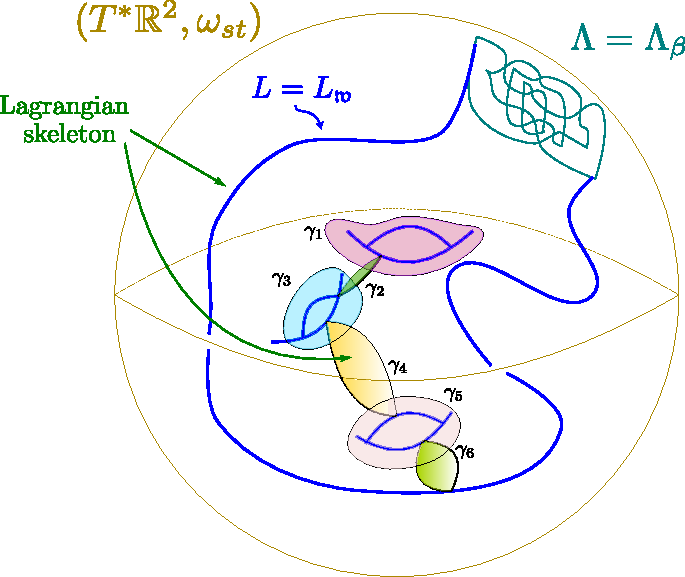
\includegraphics[scale=0.75]{figures/Filling_Merodromy2.pdf}
		\caption{A depiction of the Lagrangian surface $L_\w\sse\D^4$, constructed from $\wb$ bounding the Legendrian link $\La_\beta\sse S^3$, constructed from $\beta$. The mutable Lusztig cycles $\g_i^\w$ are geometrically realized by 1-cycles in $L_\w$ that bound embedded Lagrangian disks in the complement of $L_\w$, as it is hopefully illustrated.}
        \label{fig:Filling_Merodromy2}
	\end{figure}
\end{center}

\noindent Beyond its aesthetic value, such geometric realization of the cluster algebras $\Z[X(\beta)]$ and the weaves $\wb$ both provide new results in low-dimensional contact and symplectic topology, and informs the construction and discovery of new algebraic structures motivated by existing geometric constructions on the symplectic side. Among other instances: the introduction of weave calculus itself was originally motivated by symplectic topology in \cite{CasalsZaslow}, and the construction of cluster algebra structures on the coordinate rings of many interesting varieties, including open Richardson varieties, as illustrated in \cite{CGGLSS25}, was informed by existing results in symplectic topology.
